%%%%%%%%%%%%%%%%%%%%%%%%%%
% ABA/AB/A notes  	    %
% version 1.0            %
%%%%%%%%%%%%%%%%%%%%%%%%%%

%\documentclass[preprint,aps,floatfix]{revtex4}
%\documentclass[preprint,aps,endfloats]{revtex4}
\documentclass[twocolumn,aps,floatfix,nobibnotes]{revtex4-1}
\usepackage{graphicx,epsfig,dcolumn,bm,mathrsfs,amsmath,amssymb}
\usepackage[caption=false]{subfig}
\usepackage{color}
\bibliographystyle{apsrev}

% uncomment following three lines if using preprint endfloats
%\makeatletter
%\def\@dotsep{4.5}
%\makeatother
\graphicspath{{images/}} %Uncomment if you want to hide all figure files in a graphics/ subdirectory

\newcommand{\ud}{\mathrm{d}}
\newcommand{\fs}[1]{\textcolor{red}{#1}}
\newcommand{\jz}[1]{\textcolor{blue}{#1}}


\begin{document}

\title{The Elastic Parameters of Diblock and Triblock Copolymer Membranes}

\author{Rui Xu}
\affiliation{Department of Physics and Astronomy, McMaster University, 1280 Main Street West, Hamilton, Ontario, Canada L8S 4M1}
\author{Ashkan Dehghan}
\affiliation{Department of Physics and Astronomy, McMaster University, 1280 Main Street West, Hamilton, Ontario, Canada L8S 4M1}
\author{An-Chang Shi}
\email[]{shi@mcmaster.ca}
\affiliation{Department of Physics and Astronomy, McMaster University, 1280 Main Street West, Hamilton, Ontario, Canada L8S 4M1}
%\date{\today}

\begin{abstract}
The elastic properties of self-assembling bilayer and monolayer membranes are studied using the self-consistent field theory, using a model system of amphiphilic AB diblock copolymers and ABA triblock copolymers dissolved in hydrophilic homopolymers. We calculate the free energy of the membranes in planar, cylindrical, and spherical geometries in order to extract the bending modulus, Gaussian modulus, and line tension of the diblock and triblock membranes.  We find that the bending modulus of the triblock membrane is greater than that of the diblock membrane. We find that the Gaussian modulus and line tension of the triblock membrane suggests it is stabilized against pore formation for a greater range of copolymer architectures, and with higher pore formation energy penalties than the diblock membrane. We evaluate equilibrium bridging and looping fractions for triblock copolymers in the triblock membrane and discuss the implications for dynamically induced membrane curvature. We discuss the elastic parameters of the membranes in terms of their biological equivalents, the phospholipid bilayer membrane and the bolalipid membrane. The bolalipid membrane is exclusively found in Archaea, and we suggest it has mechanical properties that allow Archaea to survive in harsh environments.
\end{abstract}

\pacs{61.25.hk, 68.05.-n, 62.20.de}

\maketitle


%%%%%%%%%%%%%%%%%%%%%%%%%%%%%%%%%%%%%%%%%%%%%%%%%%%%%%%%%%%
\section{Introduction}
\label{sec:introduction}

Amphiphilic molecules are molecules with hydrophilic and hydrophobic components that self-assemble into mesoscopic structures when placed in a solvent. For example, amphiphilic lipids and block copolymers can self-assemble into membranes. These membranes have a unique combination of properties - they are highly flexible, yet maintain structural integrity under strong deformation \cite{lipowsky1998vesicles}. This combination of properties is crucial for many biological processes such as pore and vesicle formation. This motivates us to study the origin of the elastic parameters of the membrane; specifically the bending modulus $\kappa_M$, the Gaussian modulus $\kappa_G$, the line tension of a membrane edge $\sigma$, and the spontaneous curvature of the membrane $c_0$.

In this article, we investigate the effect of the molecular architecture of amphiphilic membrane-forming molecules. Specifically, we are interested in comparing the elastic properties of the phospholipid membrane to those of the bolalipid membrane. The phospholipid has a polar, hydrophilic head group connected to hydrophobic fatty acid chains. An amphiphilically equivalent molecule is the AB diblock copolymer, where the A block has hydrophilic properties and the B block has hydrophobic properties. The bolalipid is a bipolar molecule, consisting of two hydrophilic head groups connected by hydrophobic tail groups \cite{koga2007biosynthesis,gliozzi2002structure}. An amphiphilically equivalent molecule is the ABA triblock copolymer, which can be constructed by combining two AB diblock copolymers.

The bolalipid is exclusively found in Archaea, which are often found in extreme environments such as high temperature. It has been hypothesized that the inclusion of bolalipids into the Archaeal membrane increases the rigidity of the membrane, allowing for Archaeal membranes to maintain physiological conditions in high temperature environments \cite{oger2013adaptation,van1998essence,koga2007biosynthesis,de1986structure}. However, the origin of this purported increase in rigidity isn't fully understood. There are chemical differences between the phospholipid and the bolalipid - the bolalipid has isoprenoid fatty acid chains that may contain cyclopentane groups. Archaea also differ in that they have an S-layer, a 2D protein matrix that may confer additional stability to the Archaeal membrane. These chemical and physical characteristics, together, allow Archaea to survive in extreme environments \cite{oger2013adaptation}. However, the inclusion of all details tells us little about the exact origin of the elastic parameters of the membrane. For this purpose, we require a simple model. In our model, we solely consider hydrophilic/hydrophobic interactions in AB diblock copolymer membranes and ABA triblock copolymer membranes. This allows us to explicitly isolate the elastic effects of constraining two AB diblock copolymers to become an ABA triblock copolymer. \\
\indent Numerous experiments have been performed with phospholipid membranes to determine $\kappa_M$. The bending modulus can be obtained from a variety of experimental techniques such as monitoring thermal fluctuations in the membrane, measuring the force required to deform the membrane using a tether, and monitoring phase transitions and vesicle formation \cite{schneider1984thermal, faucon1989bending, rheinstadter2006dispersion, bo1989determination,cuvelier2005coalescence}. Few experiments have been performed with bolalipids due to their high cost and scarcity \cite{bode2008extraction}. In one experiment performed by Duwe, Kaes, and Sackman in 1990, it was found that the addition of small percentage of bolalipids (2-5 $\%$ mol) in a phospholipid bilayer would result in a significant reduction in the mean bending modulus \cite{duwe1990bending}. However, model bolaamphiphilies have been artificially synthesized to study Archaeal bolalipid membranes, and these authors found significantly higher impermeabilities to ions, significantly increased acid tolerance, and significantly increased thermal stability in their model membranes \cite{berkowitz1993new,yamauchi1993highly}. 

The properties of bolalipid membranes have been studied by finding analytical solutions to statistical mechanics models. For example, Mukhin $\&$ Kheyfets used an analytical approach to compare the free energy per bolalipid with the free energy per phospholipid pair, and found that the free energy per bolalipid was higher than the free energy per phospholipid pair \cite{mukhin2010analytical}. However, these results disagreed with a mean-field molecular theory approach taken by Longo et al., who found the opposite result \cite{longo2007stability}. Molecular dynamics simulations have been used to show the dependence of the elastic parameters bolalipid membrane on the presence of methyl groups and cyclopentane rings on the hydrophobic tail groups of the bolalipid \cite{bulacu2011silico,chugunov2014liquid}. There is some consensus in the field - most believe that the bolalipid confers additional stability to the Archaeal membrane. However, the different lipid models have led to differing results. In this work, we compare two membranes where the \textbf{only} difference between the membranes is the addition of a constraint to force pairs of AB diblock copolymers to become ABA triblock copolymers.

In order to directly calculate the elastic parameters of the AB diblock copolymer and ABA triblock copolymer membrane, we extend the method of Li et al. and Dehghan et al. to our system \cite{li2013elastic,dehghan2015line}.  We use numerical calculations with the self consistent field theory (SCFT), formulated in different geometries, to calculate the elastic moduli of the membrane. We dissolve AB diblock copolymers in A homopolymer to calculate the elastic parameters of the AB diblock copolymer membrane, and we dissolve ABA triblock copolymers in A homopolymer to calculate the elastic parameters of the ABA triblock copolymer membrane. We find the chemical potential for a tensionless membrane using a planar membrane, then construct tensionless cylindrical and spherical membranes. We use a constraint to pin the radii of the cylindrical and spherical membranes, and a constraint to form pores of different radii in a planar membrane. We then fit the SCFT free energies of these membranes to the Helfrich Model, where the membrane is represented by a 2D elastic sheet \cite{canham1970minimum,helfrich1973elastic,evans1974bending}:
\begin{equation}
F = \int dA \big[2 \kappa_M (M - c_0)^2 + \kappa_G G\big] + \sigma \int dL
\end{equation}
where $M = (c_1+c_2)/2$ is the local mean curvature, $G = c_1c_2$ is the local Gaussian curvature, where $c_1$ and $c_2$ are the principle curvatures of the membrane. In the following work, we derive elastic parameters from SCFT free energies and focus on the differences between the AB diblock and ABA triblock copolymer membranes for different hydrophilic volume fractions $f_A$. 

In addition to the elastic parameters of the ABA triblock copolymer membrane, we calculate the fraction of the copolymers in the `looped' versus bridging configuration. The bridging and looping fractions determine the strength of the coupling between the two leaflets of the membrane - a membrane with 0$\%$ looping has leaflets that are completely coupled and can be considered a monolayer membrane, while a membrane with 100$\%$ looping has leaflets that are decoupled and can be considered to be a true bilayer membrane. Processes such as phase separation into domains and shape changes in phospholipid membranes generally involve leaflets that slide relative to one another. However, in a membrane where the leaflets are strongly coupled, interleaflet sliding will be suppressed, changing the ease with which the aforementioned processes may occur. 

Previous works have suggested that the rigidity of the hydrophobic tails can significantly increase the bridging fraction, thus increasing the coupling between leaflets. However, in our model, we represent the copolymers with Gaussian chains and calculate bridging and looping fractions at equilibrium for various curved and flat membranes. Recently, Galimsyanov et al. published a set of analytical equations for the elastic deformations of bolalipid membranes, finding asymmetrical distributions of looped bolalipids between leaflets in curved membranes \cite{galimzyanov2016elastic}. Our model allows us to explicitly calculate this asymmetry as a function of membrane curvature. 

The remainder of this paper is organized as follows: Section~\ref{sec:model} describes the SCFT model of AB diblock and ABA triblock copolymer membranes and the geometric constraints used in the study. Our results on the elastic properties of the membranes and the looping versus bridging configurations of the triblock copolymer are presented in section~\ref{sec:results}, and section~\ref{sec:summary} concludes with a brief summary.



%%%%%%%%%%%%%%%%%%%%%%%%%%%%%%%%%%%%%%%%%%%%%%%%%%%%%%%%%%%
\section{Model and Method}
\label{sec:model}

In this section, we first review the theoretic framework for the calculation of the free energy of diblock and triblock copolymer membranes.
The general theory of SCFT has been well documented in several review articles
and monographs \cite{schmid1998self,fredrickson2002field,matsen2001standard,shi2004self,gompper2006soft,fredrickson2006equilibrium}, and we refer readers to them for details.
We then describe the implementation of SCFT in different geometries, which we use in order to extract the elastic constants.

\subsection{Excess free energy of a bilayer membrane}
\label{sec:freeE}

In this section, we describe the theoretical framework we use for calculating the excess free energy of a membrane using SCFT. We are interested in two types of membranes - the AB diblock copolymer membrane and the ABA triblock copolymer membrane. Both membranes are solvated by A homopolymer. These membranes exist in a volume, $V$, and the volume fraction of hydrophilic A block in the amphiphilic polymers is $f_A$. 

We set the lengths of the homopolymer and the diblock as identical, with a degree of polymerization, $N$, and we set the length of the triblock to double that of the diblock, with a degree of polymerization, $2N$. Therefore, the triblock architecture is identical to that of two diblock copolymers connected at the ends of their hydrophobic tails, and the ratio of the triblock to diblock copolymer length is $\kappa = 2$. We assume the A and B monomers are incompressible, and have the same monomer density $\rho_0$ and Kuhn length $b$. The interaction between A and B monomers is governed by the Flory Huggins Parameter, $\chi$. We will write the theory in the grand canonical ensemble, controlled by relative chemical potentials, and we use the homopolymer chemical potential as reference. The controlling parameters are the chemical potentials of the diblock, $\mu_d$ and the triblock, $\mu_t$, or the respective activities, $z_d = \exp(\mu_d)$ and $z_t = \exp(\kappa \mu_t)$.

We parameterize the contours of the copolymers using $s$, which increases from 0 to 1 for the diblock and from 0 to 2 for the triblock. We define the AB diblock copolymer as:
\begin{equation} \label{EQ:diblock}
 \nu (s) =  \begin{cases} 
      A & \text{if} \quad 0<s<f_A \\
      B & \text{if} \quad f_A<s<1
   \end{cases}
\end{equation}
and we define the symmetric ABA triblock copolymer as:
\begin{equation} \label{EQ:triblock}
 \nu (s) =  \begin{cases} 
      A & \text{if} \quad 0<s<f_A \\
      B & \text{if} \quad f_A<s< 2-f_A \\
      A & \text{if} \quad 2-f_A<s<2
   \end{cases}
\end{equation}

The Grand free energy of the system, in the mean field approximation, has the following form:
\begin{equation}
	\begin{aligned}
\frac{N \mathscr{F}}{k_B T \rho_0}  = & \int d \textbf{r} \bigg\lbrace \chi N \phi_A (\textbf{r}) 			\phi_B(\textbf{r}) - \omega_A (\textbf{r})\phi_A (\textbf{r})  \\
 &-  \omega_B(\textbf{r})\phi_B(\textbf{r}) - \xi(\textbf{r}) [ 1 -\phi_A (\textbf{r})  - \phi_B(\textbf{r})] \\
&- \psi \delta (\textbf{r} - \textbf{r}') [\phi_A (\textbf{r})  - \phi_B(\textbf{r})] \bigg\rbrace \\
&- z_d Q_d - 	\frac{z_t}{\kappa}  Q_t - Q_h
	\end{aligned}
\end{equation}
where $\phi_{\alpha} (\textbf{r})$ and $\omega_{\alpha} (\textbf{r})$ are the local concentrations and mean fields of the $\alpha$-type monomers, where $\alpha = A,B$. We introduce a Lagrange Multiplier, $\xi (\textbf{r})$, in order to enforce incompressibility. We introduce a second Lagrange Multiplier, $\psi$, to pin the membrane at a location $\textbf{r}_1$, enforced by the delta function $\delta (\textbf{r}_1 - \textbf{r})$. The term, $Q_d$ represents the single chain partition function for the diblock, while $Q_t$ and $Q_h$ represent the single chain partition functions for the triblock and homopolymer respectively. These single chain partition functions represent the configurational entropies of the chains, and can also be defined in terms of end integrated propagators:
\begin{align}
Q_d &= \int d \textbf{r} \ q_d (\textbf{r},1) \\
Q_t &= \int d \textbf{r} \ q_t (\textbf{r},2) \\
Q_h &= \int d \textbf{r} \ q_h (\textbf{r},1) 
\end{align} 
where $q_d(\textbf{r},s)$, $q_t (\textbf{r},s)$, and $q_h (\textbf{r},s)$ are the end integrated propagators, which satisfy the following modified diffusion equation:
\begin{equation} \label{EQ:Difusion_EQ}
\frac{\partial}{\partial s} q_{\beta} (\textbf{r},s)  = R_g^2 \nabla^2 q_{\beta} (\textbf{r},s) - \omega_{\small{\small{\nu(s)}}} (\textbf{r}) q_{\beta} (\textbf{r},s)
\end{equation}
where $R_g = b \sqrt{N/6}$ is the gyration radius of the copolymer chains. If $\beta = d$, then $\nu(s)$ is defined by Equation \ref{EQ:diblock}, or if $\beta = t$, then $\nu(s)$ is defined by Equation \ref{EQ:triblock}, and if $\beta = h$, then $\nu(s) = A$. The initial conditions for all propagators are $q_{\beta}(\textbf{r},0) = 1$. While the triblock and the homopolymer are symmetrical, the diblock is not. This means that we require a complementary propagator, $q_d^{\dagger} (\textbf{r},s)$ that satisfies the modified diffusion equation with the right-hand side multiplied by -1, and with the initial condition $q_d^{\dagger} (\textbf{r},1) =1$.

The SCFT method involves a mean field approximation where the free energy is calculated using a saddle-point technique where the Functional derivatives of the free energy must be found to be zero.
\begin{equation}
\frac{\delta \mathscr{F} }{\delta \phi_{\alpha}} = \frac{\delta \mathscr{F} }{\delta \omega_{\alpha}} = 
\frac{\delta \mathscr{F} }{\delta \xi} = 
\frac{\delta \mathscr{F} }{\delta \psi} = 0
\end{equation}
These functional derivatives give mean field equations for concentrations, mean fields, incompressibility, and the pinning constraint. The following equations are for concentration:
\begin{align}
\phi_A (\textbf{r}) &= \int_0^1 ds \ q_h (\textbf{r},s) q_h (\textbf{r},1-s) \nonumber \\
&+ z_d \int_0^{f_A} ds \ q_d (\textbf{r},s) q_d^{\dagger} (\textbf{r},s) \nonumber \\
&+ \frac{z_t}{\kappa} \int_0^{f_A} ds \ q_t (\textbf{r},s) q_t (\textbf{r},2-s) \nonumber \\
&+ \frac{z_t}{\kappa} \int_{2-f_A}^{2} ds \ q_t (\textbf{r},s) q_t (\textbf{r},2-s) \\
\phi_B (\textbf{r}) &= z_d \int_{f_A}^1  ds\ q_d (\textbf{r},s) q_d^{\dagger} (\textbf{r},s) \nonumber \\
&+ z_t \int_{f_A}^{2-f_A} ds \ q_t (\textbf{r},s) q_t (\textbf{r},2-s)
\end{align}
the following equations are for the mean fields:
\begin{align}
\omega_A (\textbf{r}) &= \chi N \phi_B(\textbf{r}) + \xi(\textbf{r}) - \psi \delta (\textbf{r}-\textbf{r}_1) \\
\omega_B (\textbf{r}) &= \chi N \phi_A(\textbf{r}) + \xi(\textbf{r}) + \psi \delta (\textbf{r}-\textbf{r}_1)
\end{align}
and the incompressibility and pinning constraints are:
\begin{align}
&1 = \phi_A (\textbf{r}) + \phi_B(\textbf{r}) \\
&\phi_A (\textbf{r}_1) = \phi_B (\textbf{r}_1) 
\end{align}
This set of equations is solved self-consistently using an iterative algorithm. 

We are specifically interested in the difference in free energy between a diblock or triblock copolymer membrane and a reference homogeneous system of diblock, triblock, and homopolymers. A homogeneous system has no spatial dependence, and therefore the self-consistent fields become constant (scalar) fields. The self-consistent equations can then be calculated analytically to determine the single chain partition functions, and average concentration ($\overline{\phi}_A, \overline{\phi}_B$) and mean fields ($\overline{\omega}_A, \overline{\omega}_B$). The bulk free energy, $\mathscr{F}_\text{bulk}$ is then given by the following equation:
\begin{equation}
\frac{N \mathscr{F}_{\text{bulk}} }{k_B T \rho_0} = \chi N \overline{\phi}_A \overline{\phi}_B - \overline{\omega \vphantom{+1}}_A \overline{\phi}_A - \overline{\omega \vphantom{+1}}_B \overline{\phi}_B - z_d Q_d -  \frac{z_t}{\kappa}Q_t - Q_h
\end{equation}
We are interested in the excess free energy, $\mathscr{F} - \mathscr{F}_{\text{bulk}}$ per unit area of membrane. We define this excess free energy $F$ with the following equation:
\begin{equation}
F = \dfrac{N (\mathscr{F} - \mathscr{F}_{\text{bulk}})}{k_B T \rho_0 A}
\end{equation}
where we divide by area, $A$, in order to get the excess free energy per unit area of membrane. We are also interested in a specific property of the ABA triblock copolymer  - the looping fraction. A triblock copolymer can either span the membrane in a 'bridge' conformation, or it can loop back on itself in a 'loop' configuration. These two conformations are shown in Figure \ref{fig:bridge_loop}. 

\begin{figure}[htp]
\centering
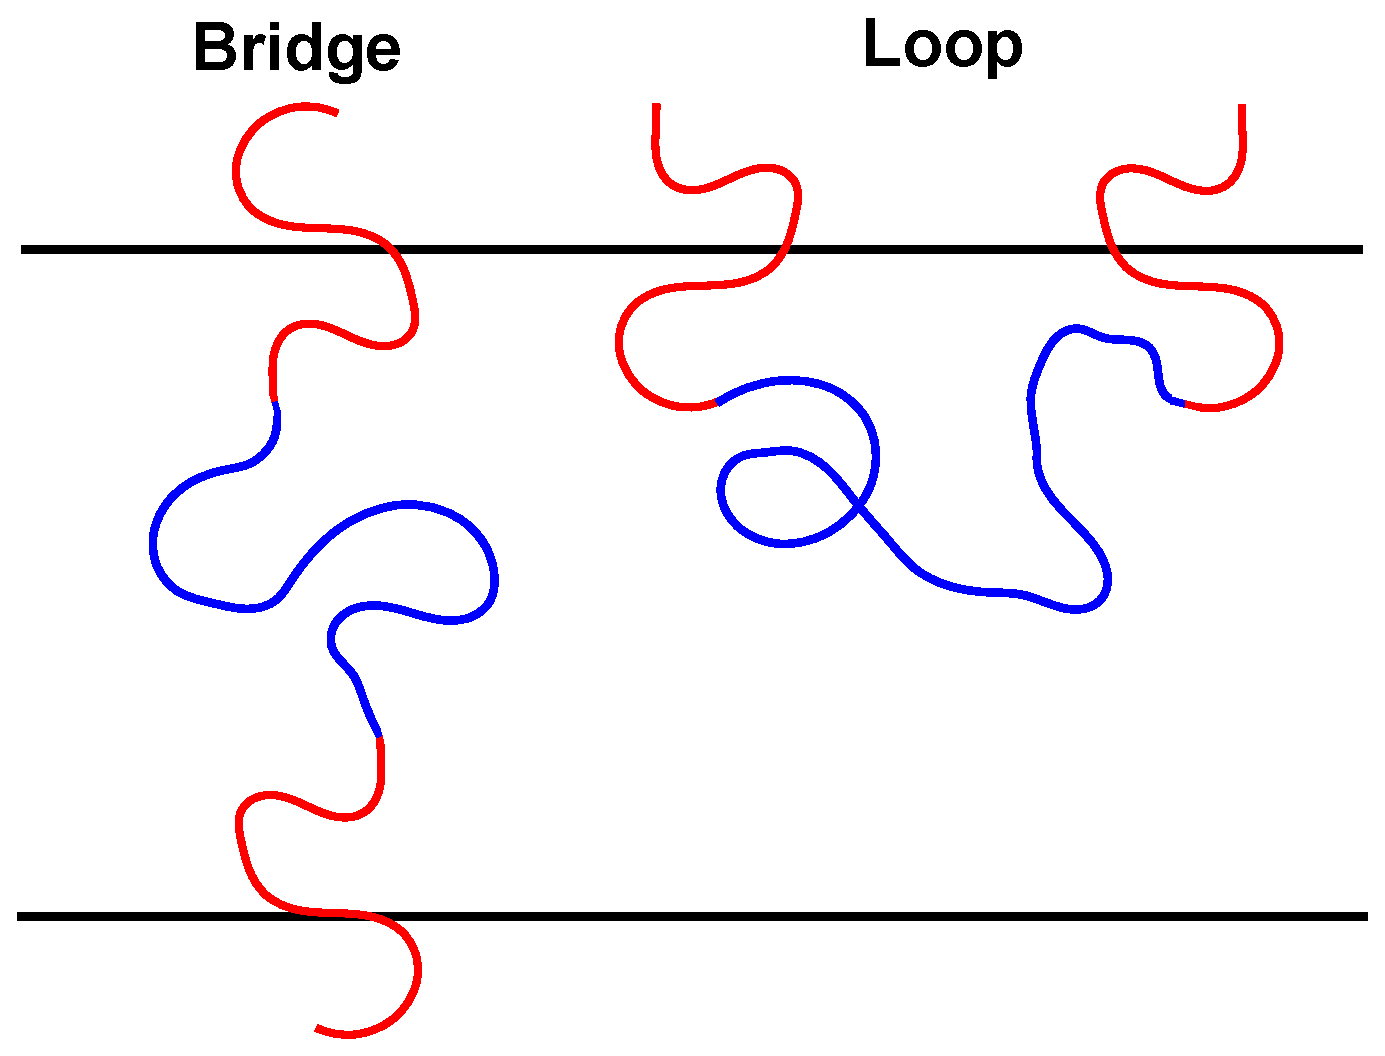
\includegraphics[width=1.0\columnwidth]{loopandbridge_polymer.eps}
\caption{An ABA triblock copolymer in `Bridge' configuration on the left, and in `Loop' configuration on the right. }
\label{fig:bridge_loop}
\centering
\end{figure}

We wish to determine the fraction of triblock copolymers that exist in the looped versus the bridge conformation. The first step involves defining a propagator with their first AB junction confined to the left half of the computation box, $\overline{q}_t^l$, and a propagator with its first AB junction confined to the right half of the computation box, $\overline{q}_t^r$:
\begin{align}
\overline{q}_t^l (\textbf{r}, f_A) &= \begin{cases}
q_t(\textbf{r},f_A) \ &\text{if} \ \ \textbf{r} < \textbf{r}_{mid} \\
0 \  &\text{otherwise}
\end{cases}\\
\overline{q}_t^r (\textbf{r}, f_A) &= \begin{cases}
q_t(\textbf{r},f_A) \ &\text{if} \ \ \textbf{r} > \textbf{r}_{mid} \\
0 \  &\text{otherwise}
\end{cases},
\end{align}
We then propagate the solution for $s \geq f_A$, and get the probability distributions $\overline{\rho}^l (\textbf{r},s)$ and $\overline{\rho}^r (\textbf{r},s)$ for the probability that the triblock loops back to the left half and right half of the computation box, respectively.
\begin{align}
\overline{\rho}^l (\textbf{r}, s) &= \frac{1}{Q_t}  \overline{q}_t^l (\textbf{r},s) q_t(\textbf{r},2-s)\\ \overline{\rho}^r (\textbf{r}, s) &= \frac{1}{Q_t} \overline{q}_t^r (\textbf{r},s) q_t(\textbf{r},2-s)
\end{align}
and the looping probabilities that a polymer that originates from the left half, $\upsilon_L^l$, and the right half. $\upsilon_L^r$, are the integrals of the probability distributions over the left-hand and right-hand sides of the computational box, respectively:
\begin{align}
\upsilon_L^l &= \frac{1}{V_{LHS}} \int_{LHS} d\textbf{r} \overline{\rho} (\textbf{r}, 2-f_A)\\
 \upsilon_L^r &= \frac{1}{V_{RHS}} \int_{RHS} d\textbf{r} \overline{\rho} (\textbf{r}, 2-f_A)
\end{align}
The bridging probabilities are simply $\upsilon_B^l = 1- \upsilon_L^l$ for a triblock that originates from the left half and $\upsilon_B^r = 1- \upsilon_L^r$. The total loop probability, $\upsilon_L$, and total bridge probability, $\upsilon_B$ are:
\begin{equation}
\upsilon_L = \frac{1}{2} (\upsilon_L^l + \upsilon_L^r), \quad \quad \upsilon_B = 1- \frac{1}{2} (\upsilon_L^l + \upsilon_L^r)
\end{equation}

\subsection{Geometrical constraints}
\label{sec:geometry}

In order to extract information on the various elastic properties, we calculate the excess free energy of a bilayer membrane in the following four geometries: (i) an infinite planar bilayer membrane, (ii) a cylindrical bilayer membrane with a radius $r$, which is extended to infinity in the axial direction, (iii) a spherical bilayer with a radius $r$, and (iv) a planar membrane with an axially symmetric pore of radius $R$.
The first three geometries can be reduced to one-dimensional systems. The planar geometry can be reduced to a one-dimensional system by assuming translational symmetry in the x and y coordinates. The cylindrical geometry can be reduced to a one-dimensional system by assuming translational symmetry in the vertical coordinate and angular symmetry in the azimuthal coordinate The spherical geometry can be reduced to a one-dimensional system by assuming angular symmetries in the azimuthal and polar coordinates. The membrane pore can be stabilized in cylindrical coordinates, and this problem can be reduced to a two-dimensional problem by assuming angular symmetry in the azimuthal coordinate. This means that we must solve the modified diffusion equation (Equation \ref{EQ:Difusion_EQ}) in one dimension and in two dimensions. We implement a Crank-Nicolson algorithm to solve the one-dimensional modified diffusion equation, and an Alternating-Direction Implicit algorithm to solve the two-dimensional modified diffusion equation \cite{press2007numerical}. 

We use the planar membrane to find the activities $z_d$ and $z_t$ that correspond to tensionless membranes. We use the cylindrical membrane to calculate the mean bending modulus, and the spherical membrane to isolate the Gaussian bending modulus. The pore configuration is use to extract the line tension of the membrane edge. 

The membranes must be stabilized in these specific geometries in order to extract the elastic parameters. We stabilite the membrane with the constraint field $\psi \delta (\textbf{r} - \textbf{r}_1) (\phi_A (\textbf{r}) - \phi_B (\textbf{r})$, which forces the concentration of hydrophilic A monomers and hydrophobic B monomers to be equal at the position $\textbf{r}_1$. We use this constraint to set the radii of the cylindrical and spherical membranes, and the radius of the membrane pore. We adjust the position $\textbf{r}$ such that the centre of the membrane (membrane neutral line), which we define as the maximum hydrophobic concentration, is centered in the middle of the computational box. We set the size of the computational box such that the fields reaches bulk values at the edges of the box, which means that the properties of the membrane we calculate are not affected by the boundary conditions of the computational box. 

We calculate the excess free energy of four types of membranes, which are denoted by $F^0$ for the planar membrane, $F^C$ for the cylindrical membrane, $F^S$ for the spherical membrane, and $F^P$ for the pore geometry. As mentioned previously, we are interested in a membrane with zero surface tension ($F_0=0$), which we find using a secant method to determine the activity $z_d$ or $z_t$ that corresponds to this state for the diblock and triblock membranes respectively.  

We now consider the curvatures of cylindrical and spherical membranes, where we define a dimensionless curvature $c = d/r$, where $d$ is the thickness of the membrane. Similarly to Katsov et al., we take the thickness of the membrane to be $d = 4.3 R_g$ \cite{katsov2004field}. The principal curvatures of a cylindrical membrane are $c_1 = d/r$ and $c_2=0$, which means that the mean curvature is $M = d/2r = c/2$ and the Gaussian curvature is $G = 0$. The principal curvatures of a spherical membrane are $c_1 = c_2 = d/r = c$, which means that the mean curvature is $M = d/r = c$ and the Gaussian curvature is $G = d^2/r^2 = c^2$. We can now write the modified Helfrich free energy for cylindrical and spherical membrane with zero surface tension, zero spontaneous curvature, and no edge:
\begin{align}
F^C &= 2 \kappa_M M^2 \quad \quad \quad \quad \ = \frac{1}{2} \kappa_M c^2 \\
F^2 &= 2 \kappa_M M^2 + \kappa_G G \quad  = (2 \kappa_M + \kappa_G)c^2
\end{align}

In high curvature regimes approaching curvatures similar to the thickness of the membrane, it is not always sufficient to rely on the second order bending moduli in the Helfrich model. In these regimes, we must also consider fourth order bending moduli, which can be written in the cylindrical and spherical geometries as $B_C$ and $B_S$ respectively. The modified Helfrich free energies for cylindrical and spherical membranes including fourth order terms are:
\begin{align}
F^C &= \frac{1}{2} \kappa_M c^2 + B_c c^4 \\
F^S &=  (2 \kappa_M + \kappa_G)c^2 + B_sc^4
\end{align}
where $B_c = \kappa_1 /16$, and $B_s = \kappa_1 + \kappa_2 + \kappa_3$. We define a natural unit for the interfacial free energy, $\gamma_{\text{int}}$ between A and B homopolymers in the limit of large $\chi N$ as:
\begin{equation}
\gamma_{\text{int}} = b k_B T\sqrt{\frac{\chi N}{6N}} 
\end{equation} 
which allows us to write the second and fourth order bending moduli as dimensionless quantities:
\begin{align}
\tilde{\kappa}_M = \frac{\kappa_M}{\gamma_{\text{int}} d^2},  \quad &\quad \tilde{\kappa}_G = \frac{\kappa_G}{\gamma_{\text{int}} d^2}, \\
\tilde{B}_c = \frac{\kappa_1}{16 \gamma_{\text{int}} d^4},  \quad &\quad \tilde{B}_s = \frac{\kappa_1+\kappa_2+\kappa_3}{\gamma_{\text{int}} d^4}
\end{align}

In pore configuration, we form a pore which has an exposed edge in a tensionless and planar membrane. The excess free energy of the pore configuration is proportional to the length of the exposed edge, and the length of the exposed edge is proportional to the radius of the pore $L = 2 \pi R$. The proportionality constant between free energy and pore radius, $\sigma$, is the line tension.
\begin{equation}
F^P = 2 \pi \sigma R
\end{equation}
We define a unit for line tension $\sigma_0 = k_B T \rho_0 d^2 /N$ to get a dimensionless line tension:
\begin{equation}
\tilde{\sigma} = \frac{\sigma}{\sigma_0}
\end{equation}

We implement these methods described in this chapter to calculate the elastic parameters of AB diblock copolymer membranes and ABA triblock copolymer membranes for a variety of parameters such as different $\chi N$, different chain fractions $f_A$, different membrane geometries, as well as for membranes consisting of blends of diblock and triblock copolymer.

\section{Results and Discussion}
\label{sec:results}

In this section, we first present the SCFT results for the second-order elastic moduli ($\kappa_M$ and $\kappa_G$) and discuss their relation to the microscopic parameter $f_A$.
We then examine highly curved bilayer membranes and demonstrate that the contribution to the free energy from the higher-order moduli can be significant.
Finally we study the bilayer membrane in disk/pore geometries and compute the line tension by varying the structure size.
Since we mainly focus on the effect of the hydrophilic volume fraction, $f_A$, on the bilayer properties, most of the results are presented for a particular interaction strength between the A and B monomers.
That is, we have fixed $\chi N=30$ unless otherwise stated.
For this intermediate segregation case, the chemical potential of the copolymer is around $\mu=4.6k_BT$ when a planar bilayer membrane becomes tensionless.
It should be noted that the interaction parameter is also important, but a change in the interaction parameter does not produce any qualitative changes to
the $f_{A}$-dependence of the elastic moduli.

\subsection{Membrane Profiles}

In this section, we demonstrate the concentration profiles that correspond to polymeric membranes. In Figures \ref{fig:ABmmbs} and \ref{fig:ABAmmbs}, we display AB diblock copolymer and ABA triblock copolymer membranes in planar, cylindrical, and spherical geometries for $f_A = 0.5$, and radii of curvature $R = 7R_g$. We fix the position of the membrane within the computational cell using the auxiliary field $\psi \delta(\textbf{r}-\textbf{r}')$ to fix the concentration profile such that $\phi_A$ = $\phi_B$ at \textbf{r}$'$. We adjust \textbf{r}$'$ to the location that corresponds to the membrane being centered in the computation box.

\begin{figure}[htp]
\subfloat[]{
   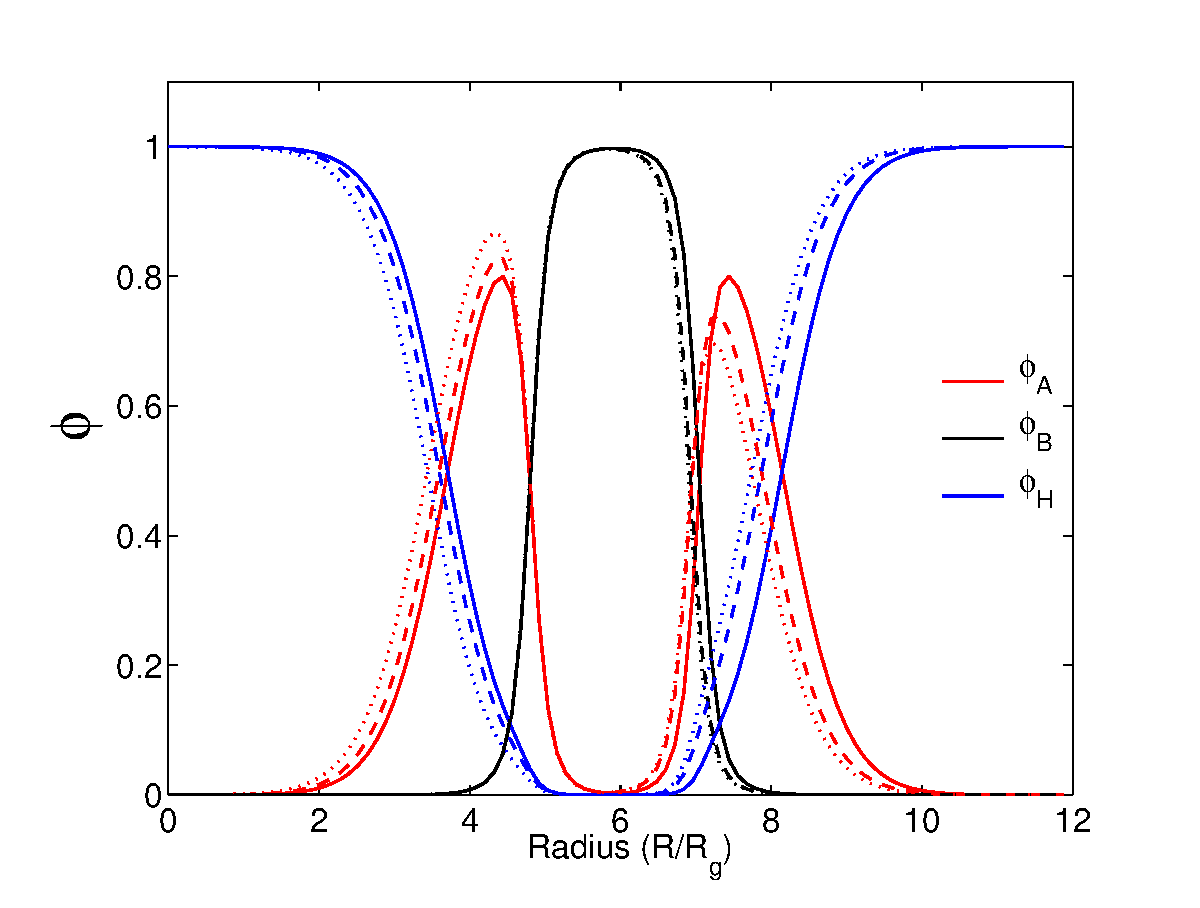
\includegraphics[clip,width=1.0\columnwidth]{ABmmb.eps}
   \label{fig:ABmmbs} 
   }
   
   
\subfloat[]{
   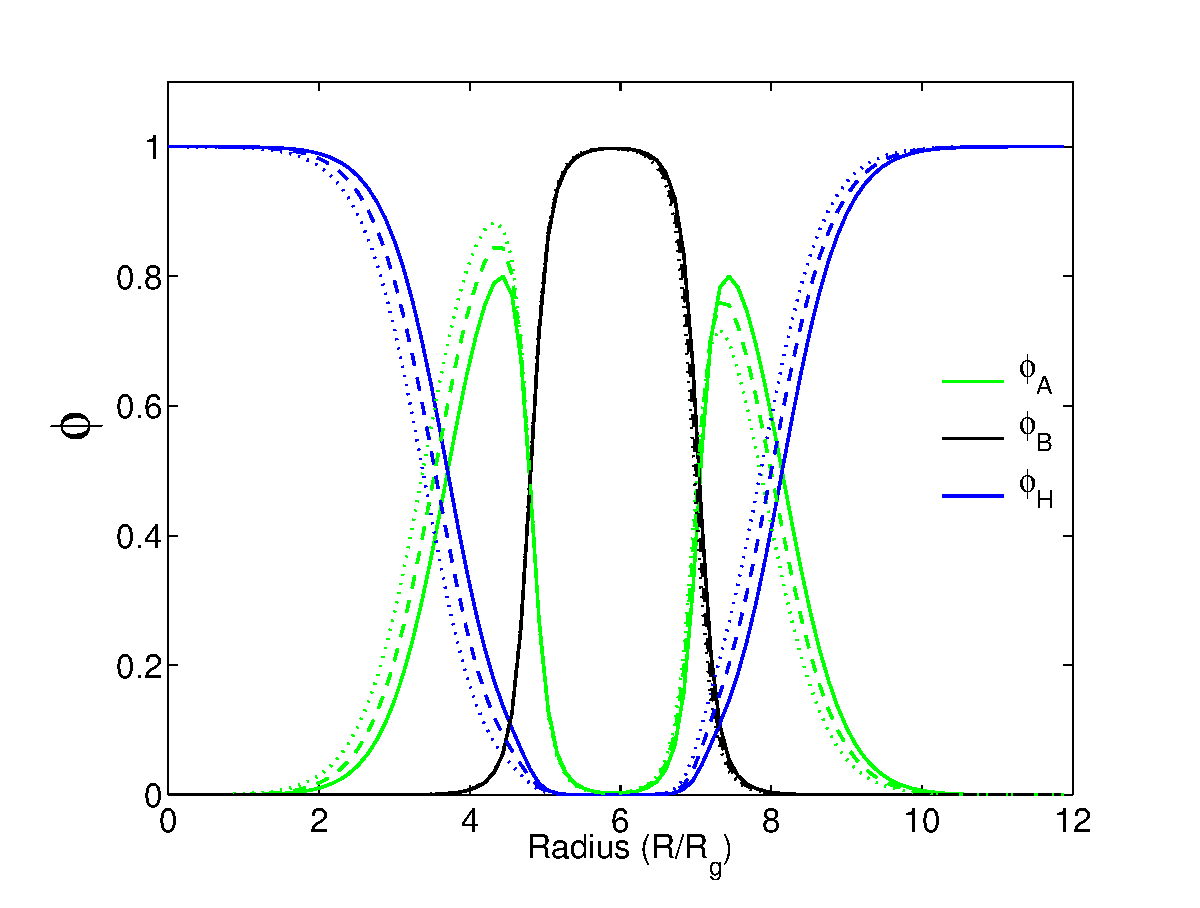
\includegraphics[clip,width=1.0\columnwidth]{ABAmmb.eps}
   \label{fig:ABAmmbs}
}
\caption[Two concentration profiles]{Concentration profiles of (a) AB diblock copolymer membranes and (b) ABA triblock copolymer membranes in planar (solid), cylindrical (dashed), and spherical (dotted) coordinates. The volume fraction, $f_A$ is set to 0.5, and the radii of cylindrical and spherical geometries are $R = 7R_g$. The asymmetry between leaflets increases from the planar to cylindrical to spherical geometries. $\phi_A$, $\phi_B$, and $\phi_H$ denote the concentrations of the A-block, B-block, and homopolymer, respectively. }
\end{figure}

The concentration profiles show increasing asymmetry between the inner and outer hydrophilic leaflets of the membranes, from the symmetric planar membrane to the highly asymmetric spherical membrane. This is due to the smaller surface area of the inner leaflet of the curved membranes, which forces the copolymers to pack more tightly, resulting in a higher local concentration relative to the outer leaflet. Another notable asymmetry that emerges is a widening of the inner hydrophilic concentration profile and a narrowing of the outer hydrophilic concentration profile. This indicates that the copolymers in the inner leaflet are stretched and the copolymers in outer leaflet are compressed relative to the planar membrane. These copolymer configurations are entropically unfavourable, resulting in an increase in free energy of the system. This increase in free energy of the system is the primary source of the bending energies of the membranes.


\subsection{Linear Elasticity: Bending and Gaussian moduli}

In this section, we demonstrate our findings for the elastic moduli of triblock copolymer monolayer membranes and diblock copolymer bilayer membranes. We isolate the elastic moduli by calculating the excess free energy of tensionless membranes in cylindrical and spherical coordinates, as a function of curvature. We then fit the free energy versus curvature results to the Helfrich model. Figure \ref{fig:FEC} demonstrates the excess free energy for tensionless diblock and triblock membranes with $f_A = 0.5$ in cylindrical and spherical coordinates. 

\begin{figure}[htp]
\centering
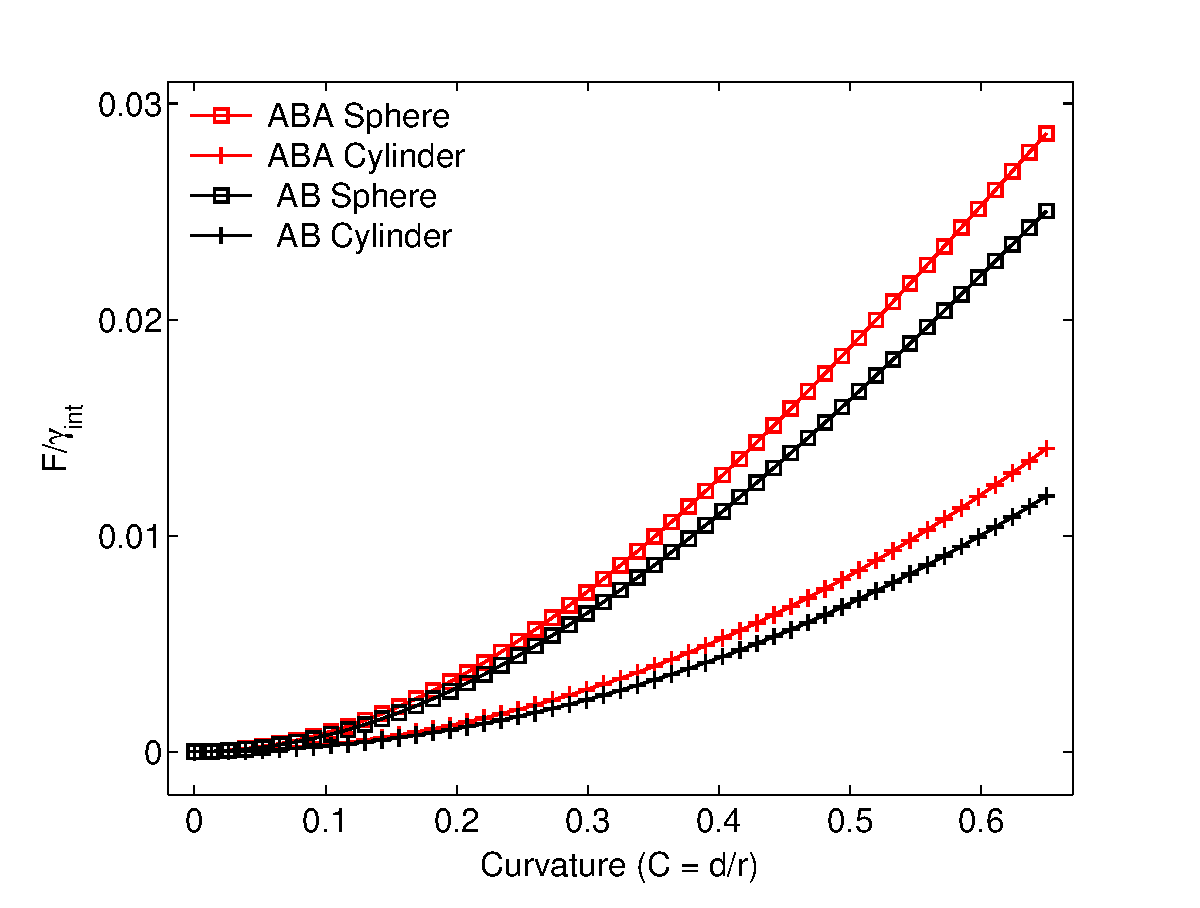
\includegraphics[width=1.0\columnwidth]{fE_C.eps}
\caption{Excess free energy for tensionless bilayer (black) and monolayer (red) membranes in cylindrical ($\square$ symbols) and spherical (+ symbols) geometries, as a function of dimensionless curvature $c = d/r$, where $d$ is the diameter of the membrane and $r$ is the radius of curvature. We set the hydrophilic chain fraction $f_A = 0.5$, and immobilize the membrane by pinning the inner leaflet such that the center of the membrane is located at the center of the computation box. }
\label{fig:FEC}
\centering
\end{figure}

In Figure \ref{fig:FEC}, it is immediately apparent that the free energy of the triblock membrane tends to be higher than that of the diblock membrane, for all tested curvatures. We limit our study to curvatures less than $c = d/r = 0.65$ to avoid contributions of higher order bending terms, in accordance with Li et. al \cite{li2013elastic}. We then perform a polynomial fit up to second order to the excess free energy. For a tensionless membrane the zeroth order term of the polynomial fit should be zero, and this is demonstrated in Figure \ref{fig:FEC} where at zero curvature the excess free energy is also zero. For a symmetrical membrane, the linear term in a polynomial fit should also be zero. This is demonstrated in Figure 3, where the slope of the excess free energy curve is zero at zero curvature. The quadratic terms, on the other hand, are non-zero and correspond to the bending modulus and the Gaussian modulus. In Figure \ref{fig:Bending_mod}, we plot the bending modulus for the diblock copolymer and triblock copolymer membranes for a range of $f_A$ that corresponds to stable diblock and triblock membranes. We show results for both $\chi N  = 30$ and $\chi N = 35$. 

\begin{figure}[htp]
\centering
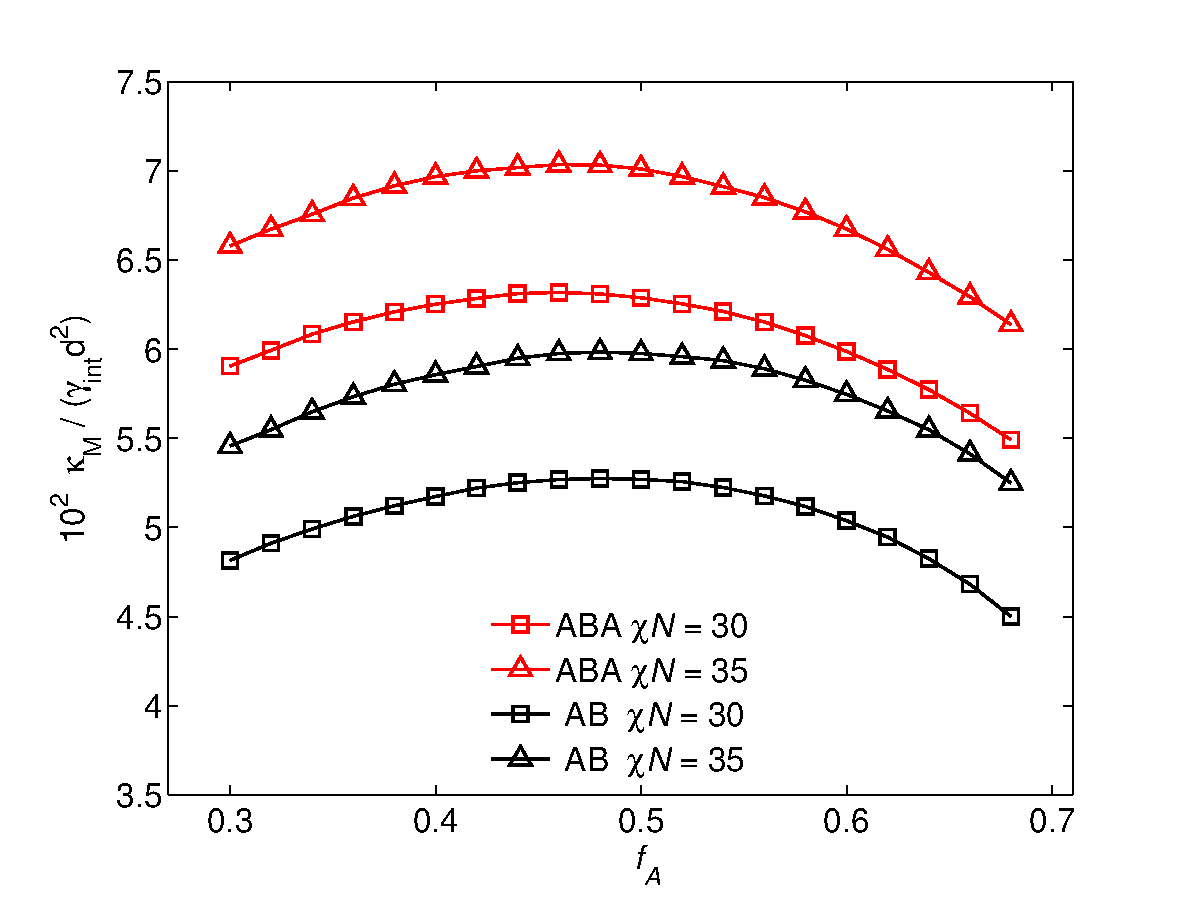
\includegraphics[width=1.0\columnwidth]{bending_mod.eps}
\caption{Dimensionless bending modulus $\kappa_M$ for bilayer (black) and monolayer (red) membranes as a function of hydrophilic chain fraction, $f_A$. We plot the result for $\chi N = 30$ and $\chi N =35$, with $\square$ and $\triangle$ symbols respectively.}
\label{fig:Bending_mod}
\centering
\end{figure}

Figure \ref{fig:Bending_mod} shows that the bending moduli of the membranes depends weakly on $f_A$, and that the maximum for the diblock membrane occurs near $f_A = 0.5$. Interestingly, this maximum is shifted towards lower $f_A$ for the triblock membrane, and occurs closer to $f_A = 0.45$. It is also immediately apparent that an increase in $\chi_N$ results in a increase in $\kappa_M$, without changing its dependence on $f_A$. Most interestingly, the bending modulus of the triblock membrane is on average 20$\%$ higher than that of the diblock membrane. This will be discussed in the context of biological membranes in the following discussion section.

In Figure \ref{fig:Gaussian_mod}, we plot the Gaussian modulus for the diblock copolymer and triblock copolymer membranes for the same range as Figure 4. In this Figure, we plot results for $\chi N = 25,30,35$ to illustrate the intersections of the Gaussian moduli near $f_A = 0.4$.


\begin{figure}[htp]
\centering
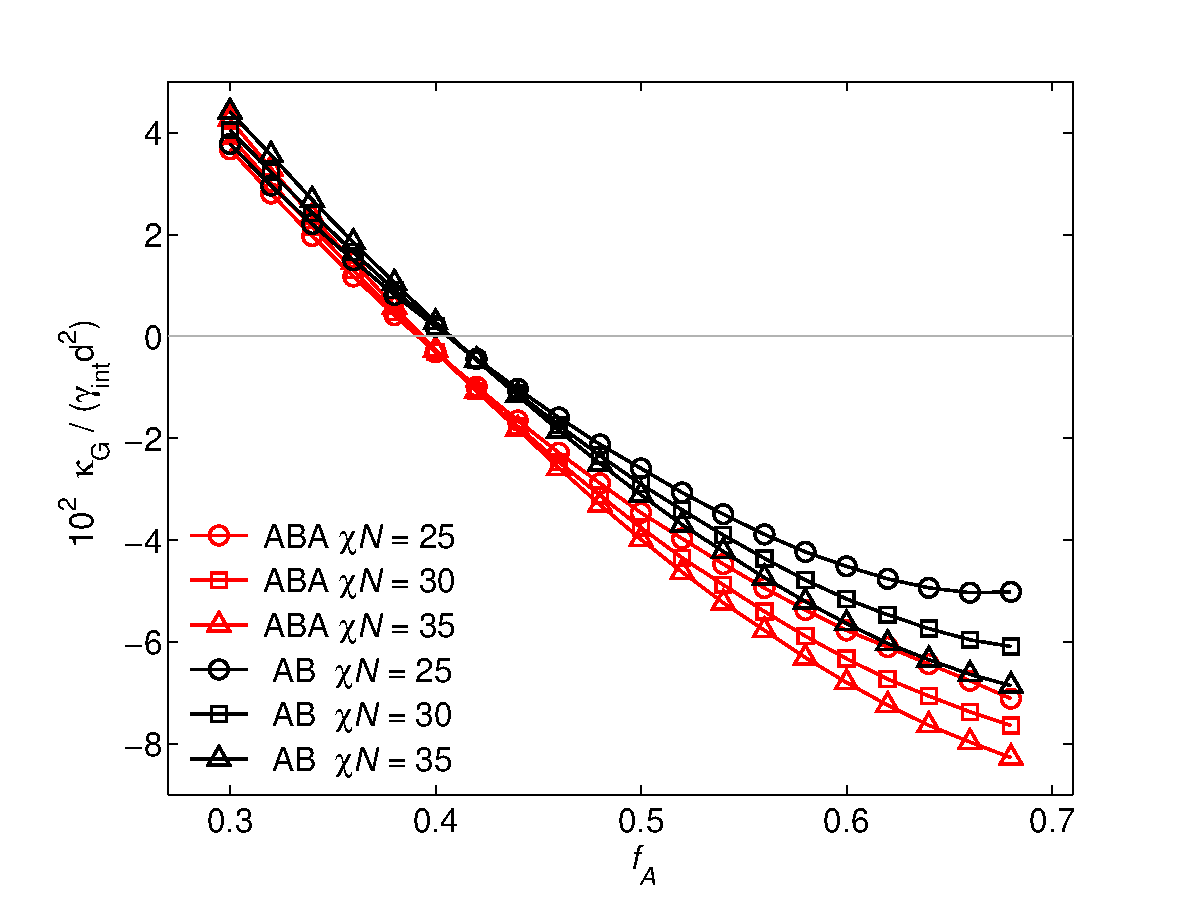
\includegraphics[width=1.0\columnwidth]{Gaussian_mod.eps}
\caption{Dimensionless Gaussian modulus $\kappa_G$ for bilayer (black) and monolayer (red) membranes as a function of hydrophilic chain fraction, $f_A$. We plot the result for $\chi N = 25,30$ and 35, with $\circ$, $\square$ and $\triangle$ symbols respectively.}
\label{fig:Gaussian_mod}
\centering
\end{figure}

Figure \ref{fig:Gaussian_mod} shows that $\kappa_G$ depends quite strongly on $f_A$ for both diblock and triblock copolymer membranes, and decreases from positive to negative as $f_A$ increases. A negative Gaussian modulus suggests a sphere geometry is preferred to a pore geometry, while a positive Gaussian modulus suggests the converse. We show that $\kappa_G$ for diblock membrane changes sign around $f_A = 0.41$, while $\kappa_G$ for the triblock membrane change sign around $f_A = 0.39$. This finding suggests that the triblock membrane is stabilized against pore formation for a greater range of chain architectures than the diblock membrane. We also plot the ratio $\kappa_G/\kappa_M$ for $\chi N = 30,35$ in Figure \ref{fig:kg_km}. 

\begin{figure}[htp]
\centering
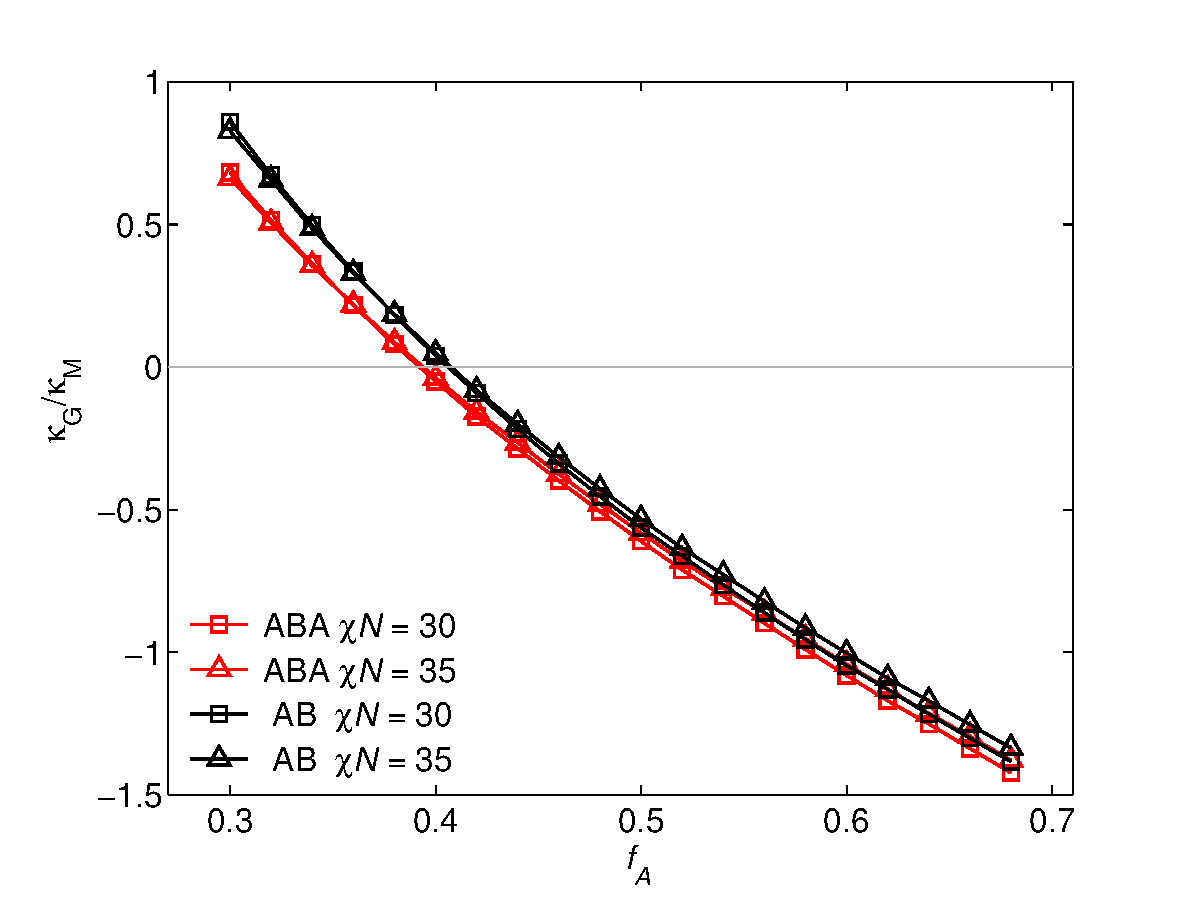
\includegraphics[width=1.0\columnwidth]{kg_km.eps}
\caption{Gaussian modulus to bending modulus ratio ($\kappa_G/\kappa_M$) for ABA triblock copolymer (red) and AB diblock copolymer (black) membranes for $\chi N = 30$ and $\chi N = 35$ with $\square$ and $\triangle$ symbols respectively.}
\label{fig:kg_km}
\centering
\end{figure}

Figure \ref{fig:kg_km} shows that the ratio $\kappa_G$/$\kappa_M$ collapses the results for different $\chi N$ onto neat, monotonically decreasing curves from approximately 1 to -1.5. This shows that the choice of the interaction parameter has minor essentially zero qualitative effect on the elastic parameters of the two types of membranes. We see that the crossing point, where $\kappa_G/\kappa_M = 0$, remains unchanged from Figure \ref{fig:Gaussian_mod}. There is little quantitative difference between $\kappa_G/\kappa_M$ for the triblock membrane and the diblock membrane other than a shift in $f_A$ dependence. 
%Comment on how this finding relates to other works

Thus far our results have solely compared the triblock copolymer membrane to the diblock membrane. However, we are also interested in membranes consisting of blends of ABA triblock and AB diblock copolymer. We define the composition of a blended membrane using the order parameter $\Omega = (\phi_d -\phi_t)/(\phi_d+\phi_t)$, where $\Omega = 1$ corresponds to the diblock copolymer membrane and $\Omega = -1$ corresponds to the triblock copolymer membrane. 

\begin{figure}[htp]
\centering
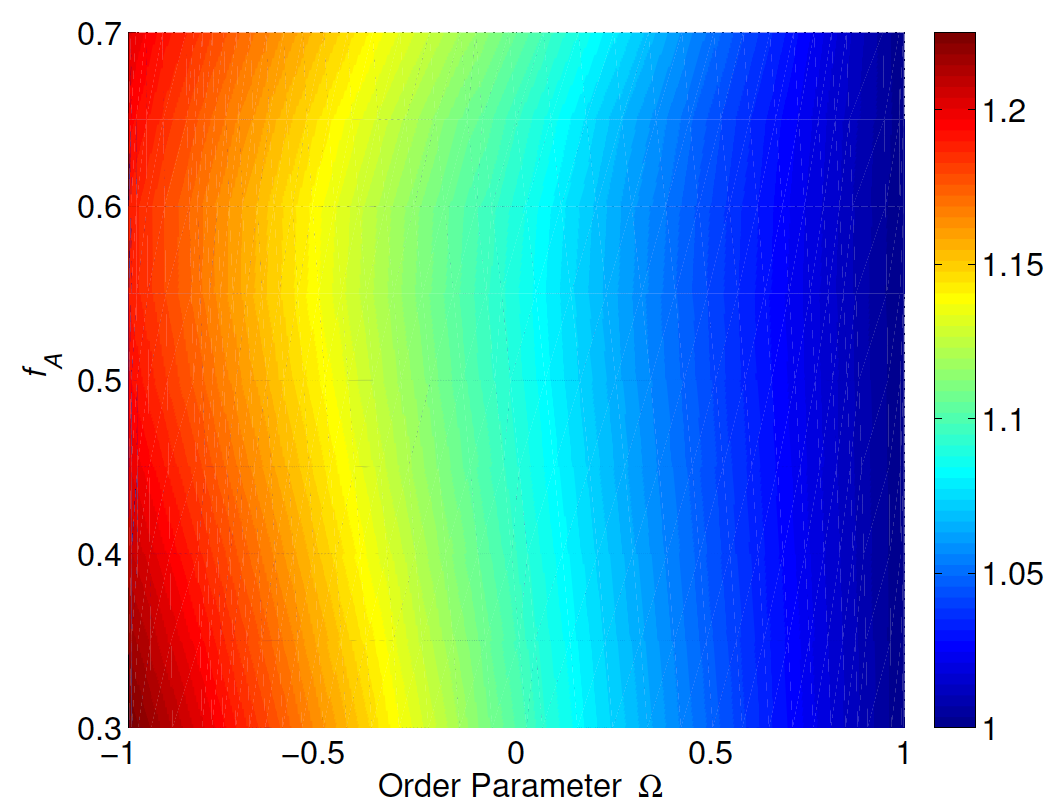
\includegraphics[width=1.0\columnwidth]{mumix_heatmap}
\caption{Bending modulus of an AB-ABA  membrane relative to the bending modulus of an AB diblock copolymer mebrane, $\kappa_M/\kappa_M^{AB}$. We represent the relative proportion of diblock to triblock using the order parameter $\Omega$, where $\Omega = 1$ represents pure diblock copolymer and $\Omega = -1$ represents pure triblock copolymer.}
\label{fig:mu_mix}
\centering
\end{figure}

Figure \ref{fig:mu_mix} shows that the bending moduli of blended ABA triblock and AB diblock copolymer membranes    decreases from the ABA bending modulus to the AB diblock modulus approximately as a linear function of the order parameter. We also observe that the relative change in bending modulus is slightly higher for lower $f_A$. This is another way of representing the $f_A$ shifted $\kappa_M$ maximum of the ABA membrane, shown in Figure \ref{fig:Bending_mod}. As expected, changing the order parameter from -1 to 1 results in a shift in $\kappa_G$ from the ABA triblock result to the AB diblock result shown in Figure \ref{fig:Gaussian_mod}.

\subsection{Line Tension of a Membrane Edge}

In this section, we present and discuss our results for the line tension of ABA triblock copolymer and AB diblock copolymer membranes. When a pore is formed in a membrane, the lipids reorient themselves to avoid unfavourable interactions between the solvent and the hydrophobic tails. An analogous process occurs in diblock and triblock copolymer membranes, where the copolymers reorient themselves to avoid any interface between the homopolymer solvent and the hydrophobic B blocks of the membranes. However, this reorientation comes at the cost of a decreasing the configurational entropy of the polymers in the membrane `edge'. This energy penalty is the main contributor to the line tension of the pore. We calculate line tension by forming a pore in a planar membrane, and assume that the pore has azimuthal symmetry. Figure \ref{fig:Pore} demonstrates the pore geometry, and we define the radius `$\textbf{R}$' of the pore as the distance from the center of the pore to the pinned location $r_1$, which is enfored by the Lagrange Multiplier $\psi \delta (\textbf{r}_1 - \textbf{r})[\phi_A(\textbf{r}) - \phi_B(\textbf{r})]$. 

\begin{figure}[htp]
\centering
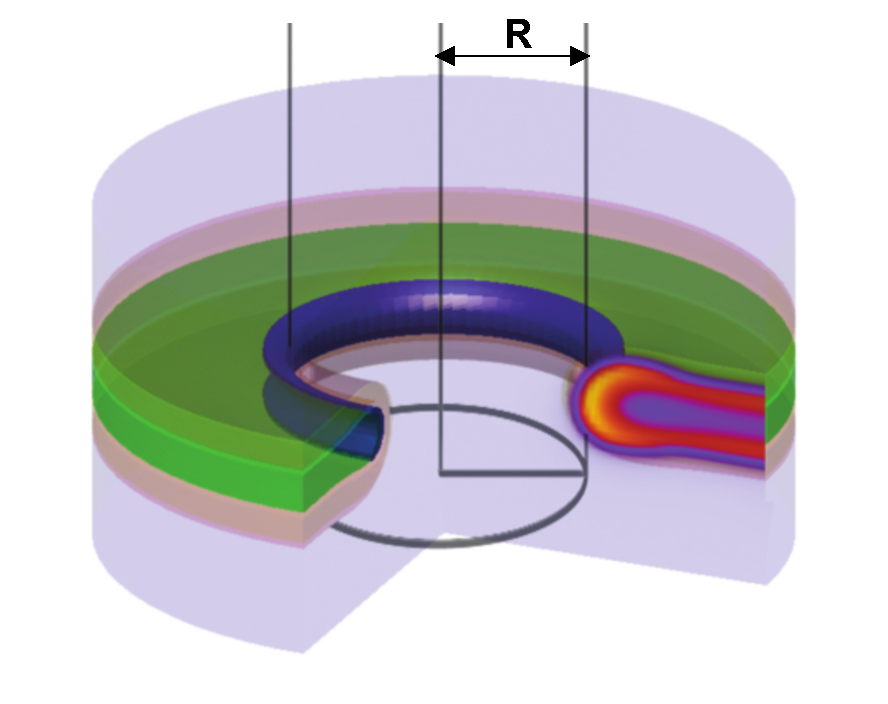
\includegraphics[width=1.0\columnwidth]{Pore.eps}
\caption{We extract line tension by calculating the excess free energy of a pore in a planar membrane, as a function of pore radius. The solvent is blue, the hydrophilic A blocks are red, and the hydrophobic B blocks are green. The inset heatmap shows the A concentration, from  $\phi_A \approx 1.0$ in yellow to $\phi_A \approx 0$ in purple.}
\label{fig:Pore}
\centering
\end{figure}

We begin by calculating the chemical potential corresponding to tensionless planar membranes. We then proceed to calculate the excess free energy of pores of different radii. Figure \ref{fig:Pore_FE} demonstrates the relationship between the free energy of a Pore and the radius of the pore, $F^P = 2 \pi \sigma R$, for different $f_A$, and for $\chi_N = 30$. 

\begin{figure}[htp]
\centering
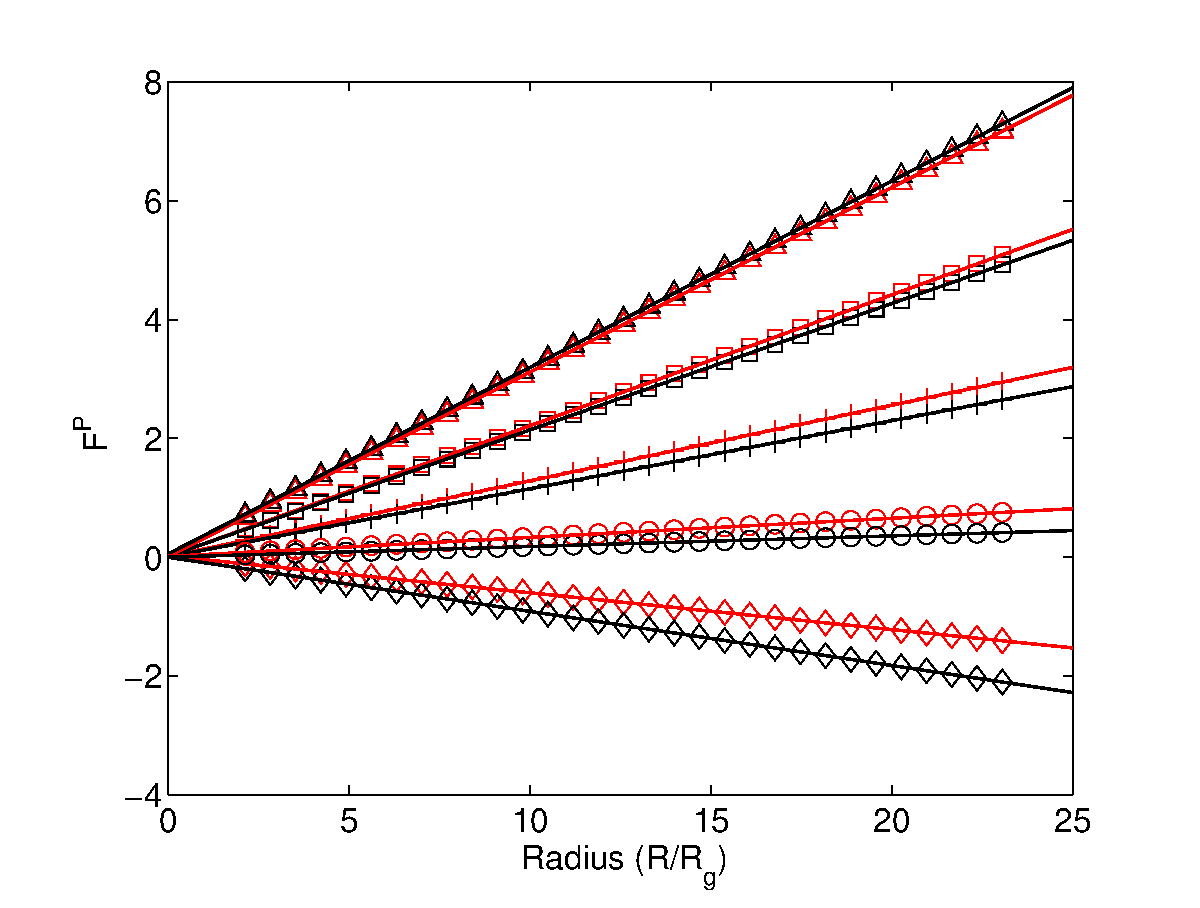
\includegraphics[width=1.0\columnwidth]{Pore_fE_R.eps}
\caption{Excess free energy for a pore in a planar bilayer membrane, as a function of pore radius for $f_A = 0.3,0.4,0.5,0.5,0.7$, denoted by $\bigtriangleup$, $\square$, $+$, $\circ$, and $\lozenge$ respectively.}
\label{fig:Pore_FE}
\centering
\end{figure}

As we can see, the line tension for both ABA triblock and AB diblock membranes decrease as $f_A$ increases from positive values at lower $f_A$ to negative values for $f_A$ greater than approximately 0.6. It is also clear from these results that the excess free energies of the ABA triblock pores tends to be higher than the excess free energies of the AB diblock pores, suggesting that pore formation in ABA triblock membranes tends to be less favourable than in AB diblock membranes. We then extract the line tension by fitting the data shown in Figure \ref{fig:Pore_FE} with a linear least squares fit. The resultant data is shown in Figure \ref{fig:Line_tension}. 

\begin{figure}[htp]
\centering
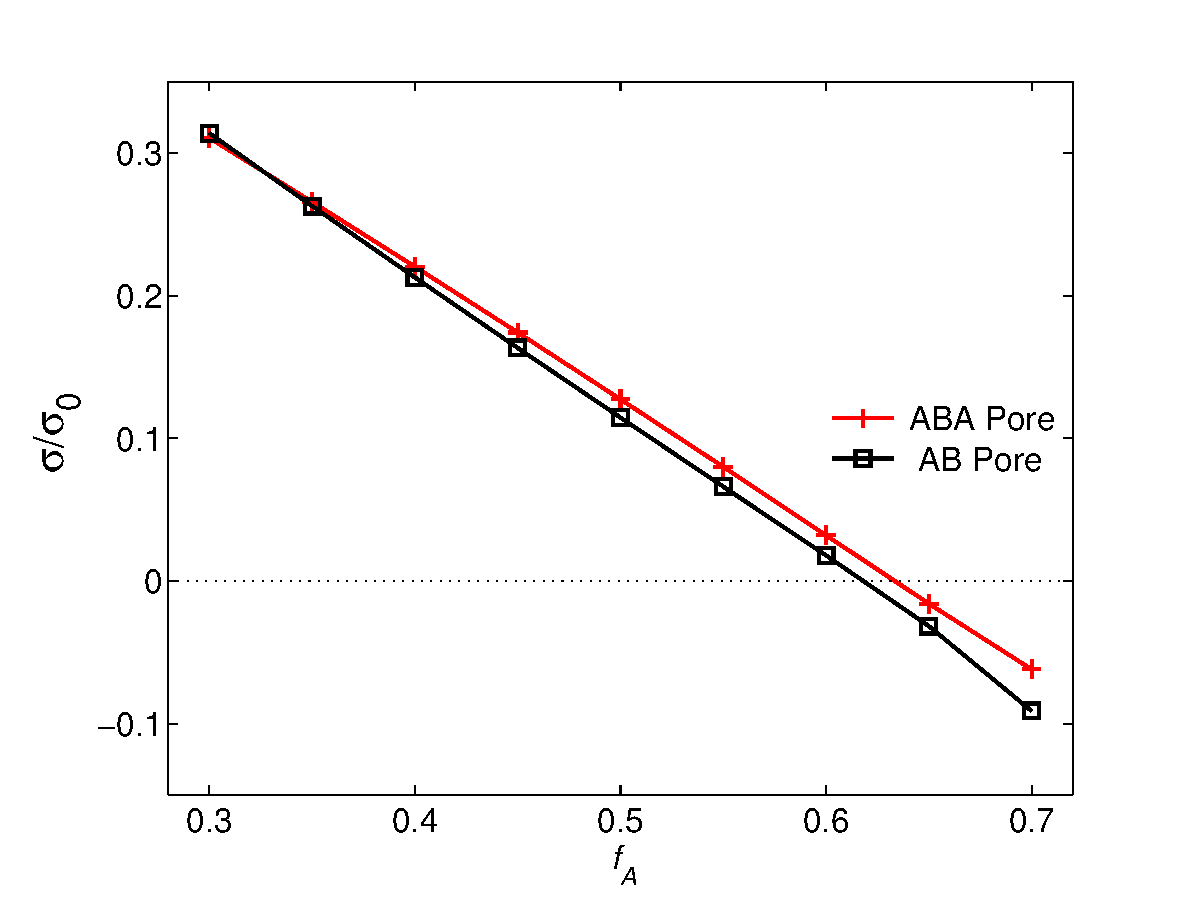
\includegraphics[width=1.0\columnwidth]{line_tension}
\caption{Dimensionless line tension for ABA triblock copolymer membranes (red) and AB diblock copolymer membranes (black), calculated from the free energies of pores in planar membranes.}
\label{fig:Line_tension}
\centering
\end{figure}

The line tensions for the ABA triblock and AB diblock copolymer membranes, as a function of $f_A$ are shown in Figure \ref{fig:Line_tension}. The line tensions for the triblock membrane and diblock membrane at $f_A \approx 0.3$ are approximately equivalent. However, as $f_A$ increases, the line tensions for the different membranes diverge, and line tension in the triblock membrane tends to be slightly higher than in the diblock membrane. This divergence results in different cross-over points from positive to negative line tensions - in the diblock membrane, then $\sigma = 0$ at approximately $f_A = 0.62$, while in the triblock membrane this occurs at approximately $f_A = 0.64$. The increased line tension of the triblock membrane for large $f_A$ originates from the reduced conformational degrees of freedom for a triblock copolymer in the looped configuration due to the shortened $B$ block. The shift in the $f_A$ dependence of the cross-over point is quite similar to that calculated for the Gaussian modulus (Figure \ref{fig:Gaussian_mod}). In both cases, we found that the triblock membrane was stabilized against pore formation for a range $\Delta f_A \approx 0.02 $ larger than the diblock membrane. 

The qualitative behaviour of line tension in the two types of membranes were the same. In both cases, we have regions of negative line tension corresponding to lipids that stabilize the pores, a result that has been observed experimentally and in molecular dynamics simulations \cite{karatekin2003cascades,de2006coarse}. However, most lipids have hydrophilic chain fractions less than 0.5, which means that most biological membranes are stabilized against pore formation. The difference between diblock and triblock copolymer membrane line tensions at low $f_A$ is smaller than at large $f_A$, which means that based on this result we would expect there to be little difference in line tensions for phospholipid and bolalipid membranes. 


\subsection{Looping Fraction}

In this section, we investigate the looping fraction of ABA triblock copolymers in pure ABA triblock copolymer membranes and discuss several implications of the findings. An ABA triblock copolymer can assume two states - the loop state and the bridge state. Looping fractions have been investigated in the context of lamellar, cylindrical, and spherical ABA triblock morphologies by Matsen $\&$ Thompson, who found looping fractions of $55 - 60\%$, $35-40\%$, and $20-25\%$ for the three respective morphologies \cite{matsen1999equilibrium}. We calculate the looping fractions for the inner and outer leaflets of ABA triblock copolymer membranes at different curvatures, and for a range of $f_A$. We find looping fractions that are highly dependent on membrane curvature, and the results are shown in Figure \ref{fig:loop_fraction}. 

\begin{figure}[htp]
\centering
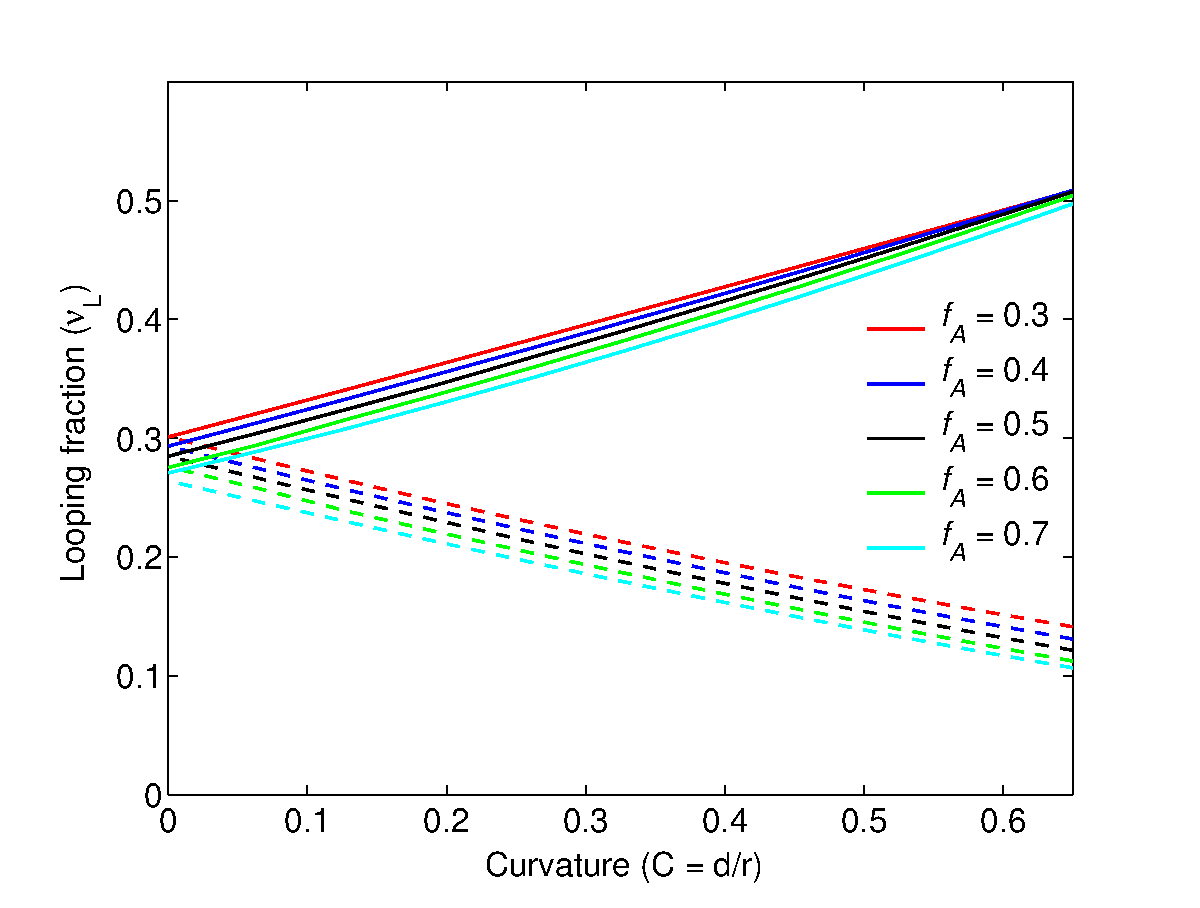
\includegraphics[width=1.0\columnwidth]{loop_fraction.eps}
\caption{Inner (dashed lines) and outer (solid lines) leaflet looping fractions for ABA triblock copolymer membranes as a function of curvature for various $f_A$. We calculate the looping fractions in spherical membrane geometry; the results are qualitatively the same in cylindrical geometry.}
\label{fig:loop_fraction}
\centering
\end{figure}

In Figure \ref{fig:loop_fraction}, we see that the looping fraction of the inner leaflet decreases and the looping fraction of the outer leaflet increases as membrane curvature increases. As one would expect, there is no difference in looping fraction between leaflets for planar membranes ($C = 0$). We find that the bridge configuration ($\nu_b = 1 - \nu_L$) dominates, a result that matches experimental results for bolalipid bridging fractions \cite{thompson1992tetraether,brownholland2009phase,holland2008bolalipid}. Similarly to the concentration asymmetries shown in Figures \ref{fig:ABmmbs} and \ref{fig:ABAmmbs}, this finding is due to the relative decrease in inner leaflet area and increase in outer leaflet area as curvature increases. The chain architecture $f_A$ has a minor influence on the looping fraction, with higher $f_A$ resulting in incrementally lower looping fractions. 

This result shows that the leaflets of the triblock copolymer membrane are strongly coupled, with bridging fractions around 70$\%$. This prevents inter-leaflet shear, and may significantly affect the kinetics of processes such as vesicle budding, phase separation, and other morphological membrane changes. These differences are beyond the scope of this thesis, but could potentially be investigated using dynamical SCFT \cite{grzetic2014statistical}.

%%%%%%%%%%%%%%%%%%%%%%%%%%%%%%%%%%%%%%%%%%%%%%%%%%%%%%%%%%%
\section{Summary}
\label{sec:summary}

We have calculated and contrasted the elastic parameters of AB diblock copolymer and ABA triblock copolymer membranes, where the triblock copolymers are analogous to two diblock copolymers connected at the ends of their respective B blocks. We investigated the bending modulus, the Gaussian modulus, and the pore line tension of the two types of membranes using Equilibrium self-consistent field theory. We found significant differences in the elastic parameters of the two types of membranes that are solely the result of this connection between B blocks. \\
\indent We calculated a 20$\%$ increase in bending modulus for triblock membranes relative to diblock membranes; a result that was largely independent of the volume fraction of the hydrophilic A block, $f_A$. By tuning the relative concentration of diblock to triblock copolymer, we showed that bending modulus increases proportionally to the concentration of triblock copolymer.  \\
\indent We calculated the Gaussian modulus for both membranes and found both to be monotonically decreasing functions of $f_A$, from positive to negative. However, it was found that the triblock membrane had a Gaussian modulus that crossed from positive to negative at $f_A \approx 0.39$, whereas the diblock membrane had a Gaussian modulus that crossed at $f_A \approx 0.41$. This suggests that the triblock membrane is stabilized against pore formation for a larger range of $f_A$ than the diblock membrane. \\
\indent We calculated the line tension for both membranes, and found similar, monotonically decreasing line tensions as $f_A$ increased. At that at low $f_A$ there was very little difference in line tension between the membranes, however, as we increased $f_A$, the line tension of the triblock membrane tended to be higher. We found that the crossing point from positive to negative line tensions occurred near $f_A = 0.62$ in the diblock membrane, whereas this crossing point occurred near $f_A = 0.64$ in the triblock membrane. This result, in combination with the difference in Gaussian modulus,  shows that pore formation is less favourable in a triblock copolymer membrane in terms both the topological transition and the energy penalty to maintain the pore geometry. \\
\indent We calculated the looping fractions in spherical ABA triblock copolymers for different curvatures. At small curvatures, we found looping fractions to be approximately 30$\%$, which is similar to experimental results for bolalipid membranes \cite{thompson1992tetraether,brownholland2009phase,holland2008bolalipid}. As we increased curvature, we found that the looping fraction would decrease in the inner membrane leaflet, and increase in the outer membrane leaflet. This suggests that in a dynamically bending membrane, the lateral diffusion and flip-flop rates of the triblock copolymer becomes especially important because unlike the phospholipid membrane, the leaflets of the bolalipid membrane are strongly coupled and cannot slide against each other. Although comparisons of interleaflet viscosity are beyond the scope of this thesis, this phenomenon could potentially be investigated using dynamical self-consistent field theory \cite{grzetic2014statistical}.\\
\indent The results comparing the  elastic parameters of AB diblock copolymer and ABA triblock copolymer membranes are more rigid and less able to form pores. We proposed that we could extend these results to biological membranes, in order to compare the properties of phospholipid membranes to bolalipid membranes. Biological membranes tend to be extremely complex systems, with an assortment of lipids, proteins, steroids and oligosaccharides. However, the most fundamental property of the membrane is the amphiphilicity of its lipid constituents \cite{singer1972fluid}. By representing the phospholipid and the bolalipid as AB diblock copolymers and ABA triblock copolymers and comparing the elastic parameters of the membranes, we can understand the effect of linking to diblock copolymers to form a triblock copolymer membrane will have. This is analogous to joining two phospholipids together at the fatty acid tails and then investigating the elastic parameters of the membrane. While there are other properties of the bolalipid to consider, such as the isoprenoid chains and cyclopentane rings in bolalipids, these properties have been shown to increase the rigidity of the lipid, which would in turn increase the magnitude of the elastic parameters calculated in this thesis \cite{bulacu2011silico,chugunov2014liquid}. Therefore, our estimates form a lower limit for any expected change in elastic properties of bolalipid membranes. \\
\indent It has long been hypothesized that the bolalipid confers additional stability to biological membranes, and that bolalipid membranes play an important role in allowing Archaea to survive in hostile environments such as high temperature and high pressure. We believe that this extension from amphiphilic block copolymer membrane to phospholipid and bolalipid membranes gives insight into the behaviour of both types of membranes, and supports the homeoviscous adaptation theory that suggests bolalipids are included to increase thermal and mechanical stability in Archaeal membranes. Understanding the properties of the bolalipid membrane is also important for various biotechnological applications \cite{jacquemet2009archaeal,bulacu2011silico,de2014cell}.\\
\indent This work has extended the methodology introduced by Li et al. to ABA triblock copolymer membranes, and demonstrated the precision with which the elastic parameters of different amphiphilic block copolymer membranes can be calculated and compared. By assuming symmetries in planar, cylindrical, spherical, and pore membrane geometries, we reduce the computational cost of solving the self-consistent equations for these systems to calculations that can easily be performed on a single cpu and that will converge to the equilibrium solution within minutes. This framework allows for the membrane parameter space to be investigated quickly and computationally inexpensively. Extensions to charged systems, dynamical systems, and systems with a wider range of copolymer morphologies are feasible, and provide interesting directions for future research. There are many questions that can be answered using this method, and potential future directions include investigating asymmetrical triblock copolymers, and blends of diblock and triblock copolymers with $\kappa \neq 2$. Another interesting question is how other constituents of biological membranes such as cholesterol might affect the elastic properties of membranes. There are many avenues for using SCFT to calculate the elastic parameters of membranes, making this an exciting and invigorating subject for future work.






%%%%%%%%%%%%%%%%%%%%%%%%%%%%%%%%%%%%%%%%%%%%%%%%%%%%%%%%%%%
 \begin{acknowledgments}
We acknowledge support from the Natural Sciences and Engineering Research Council (NSERC) of Canada through Discovery and CREATE programme.
This work was made possible by the facilities of the Shared Hierarchical Academic Research Computing Network (SHARCNET:www.sharcnet.ca) and Compute/Calcul Canada.
 \end{acknowledgments}



%%%%%%%%%%%%%%%%%%%%%%%%%%%%%%%%%%%%%%%%%%%%%%%%%%%%%%%%%%%

%%%%%%%%%%%%%%%%%%%%%%%%%%%%%%%%%%%%%%%%%%%%%%%%%%%%%%%%%%%
%\bibliography{line}
%\bibliographystyle{aipauth4-1}
\bibliographystyle{unsrtnat}

\bibliography{bibl}


% uncomment the following lines if using preprint endfloats
%\listoffigures

\end{document}
